\documentclass[12pt, fleqn]{article}
\usepackage[top=0cm, bottom=0cm, left=0cm, right=0cm, paperheight=16000pt]{geometry}
\usepackage{amsmath, amssymb, amsthm, bm, setspace, cmbright, tikz, algpseudocode, algorithm, xfrac}
\setlength{\parindent}{0pt}
\begin{document}
\setstretch{1.25}
\pagestyle{empty}
%dontshow
\gdef\Res{\operatorname{Res}}
\gdef\diff{\mathop{}\!\mathrm{d}}

\(f\)

\(G\)

\(a_1,a_2,\dots,a_m\)

\(\gamma\)

\(a_k\)

\(\gamma\approx 0\)

\[
    \frac{1}{2\pi i} \int\limits_\gamma f\Bigl(x^{\mathbf{N}\in\mathbb{C}^{N\times 10}}\Bigr)
    = \sum_{k=1}^m n(\gamma;a_k)\Res(f;a_k)\,.
\]

\(\mathbb{C}\)

\(G^-\)

\[
    \max\{\, |f(z)|:z\in G^- \,\} = \max\{\, |f(z)|:z\in \partial G \,\}\,.
\]

\(\iiint\limits_{Q}f(x,y,z) \diff x \diff y \diff z\)

\(\prod_{\gamma\in\Gamma_{\bar{C}}}\partial(\tilde{X}_\gamma)\)

\[
    \iiiint\limits_{Q}f(w,x,y,z) \diff w \diff x \diff y \diff z
  \leq
  \oint_{\partial Q} f'\Biggl(\max\Biggl\{
  \frac{\Vert w\Vert}{\vert w^2+x^2\vert};
  \frac{\Vert z\Vert}{\vert y^2+z^2\vert};
  \frac{\Vert w\oplus z\Vert}{\vert x\oplus y\vert}
  \Biggr\}\Biggr)\,.
\]

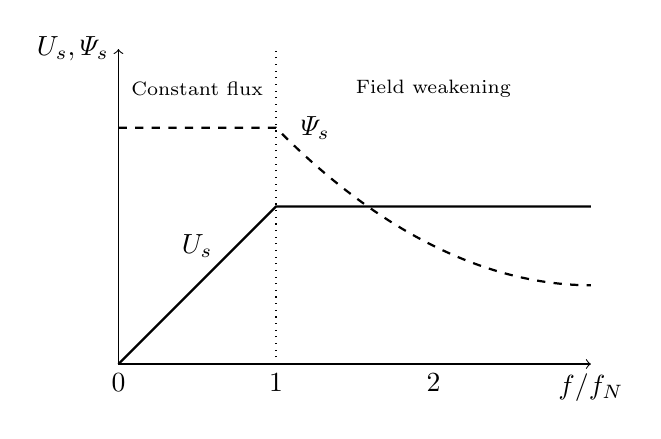
\begin{tikzpicture}
% horizontal axis
\draw[->] (0,0) -- (6,0) node[anchor=north] {$f/f_N$};
% labels
\draw   (0,0) node[anchor=north] {0}
        (2,0) node[anchor=north] {1}
        (4,0) node[anchor=north] {2};
% ranges
\draw   (1,3.5) node{{\scriptsize Constant flux}}
        (4,3.5) node{{\scriptsize Field weakening}};

% vertical axis
\draw[->] (0,0) -- (0,4) node[anchor=east] {$U_s,\varPsi_s$};
% nominal speed
\draw[dotted] (2,0) -- (2,4);

% Us
\draw[thick] (0,0) -- (2,2) -- (6,2);
\draw (1,1.5) node {$U_s$}; %label

% Psis
\draw[thick,dashed] (0,3) -- (2,3) parabola[bend at end] (6,1);
\draw (2.5,3) node {$\varPsi_s$}; %label

\end{tikzpicture}

\begin{algorithm}
\caption{An algorithm with caption}\label{alg:cap}
\begin{algorithmic}
\Require $n \geq 0$
\Ensure $y = x^n$
\State $y \gets 1$
\State $X \gets x$
\State $N \gets n$
\While{$N \neq 0$}
\If{$N$ is even}
    \State $X \gets X \times X$
    \State $N \gets \frac{N}{2}$  \Comment{This is a comment}
\ElsIf{$N$ is odd}
    \State $y \gets y \times X$
    \State $N \gets N - 1$
\EndIf
\EndWhile
\end{algorithmic}
\end{algorithm}

\end{document}